\section{MoCho}\label{sec:cityscope-mocho}
{
    \subsection{Introduction}
    {
        Understanding the impact of city-planning on mobility habits of urban dwellers is fundamental to well functioning cities. Nevertheless, it is challenging to predict, communicate, and demonstrate the correlation between minor urban interventions and metropolitan scale mobility mode-choices (MC). CityScope `MoCho' is a real-time MC modeling and prediction module that simulates MC of individuals in a metro region, in response to small-scale urban-design transformation. The prediction models consider individual characteristics and attributes of available alternatives, and are calibrated using survey data. To explore MoCho MC predictions, users interact with the CityScope TUI which triggers new MC predictions, alongside their impacts based on land-use, density or spatial proximity. As a case-study, MoCho has been developed to simulate MC for the Boston metro area, focusing on a 14 acres development site in Kendall Sq. (see Section \eqref{appendix:playground}). The choice model was fitted and the parameters showed significant associations with a range of explanatory variables, including travel times, residential and employment densities, as well as personal attributes like age, gender, education-level and home-ownership.
    }



    \begin{figure}[!htb]
        \centering
        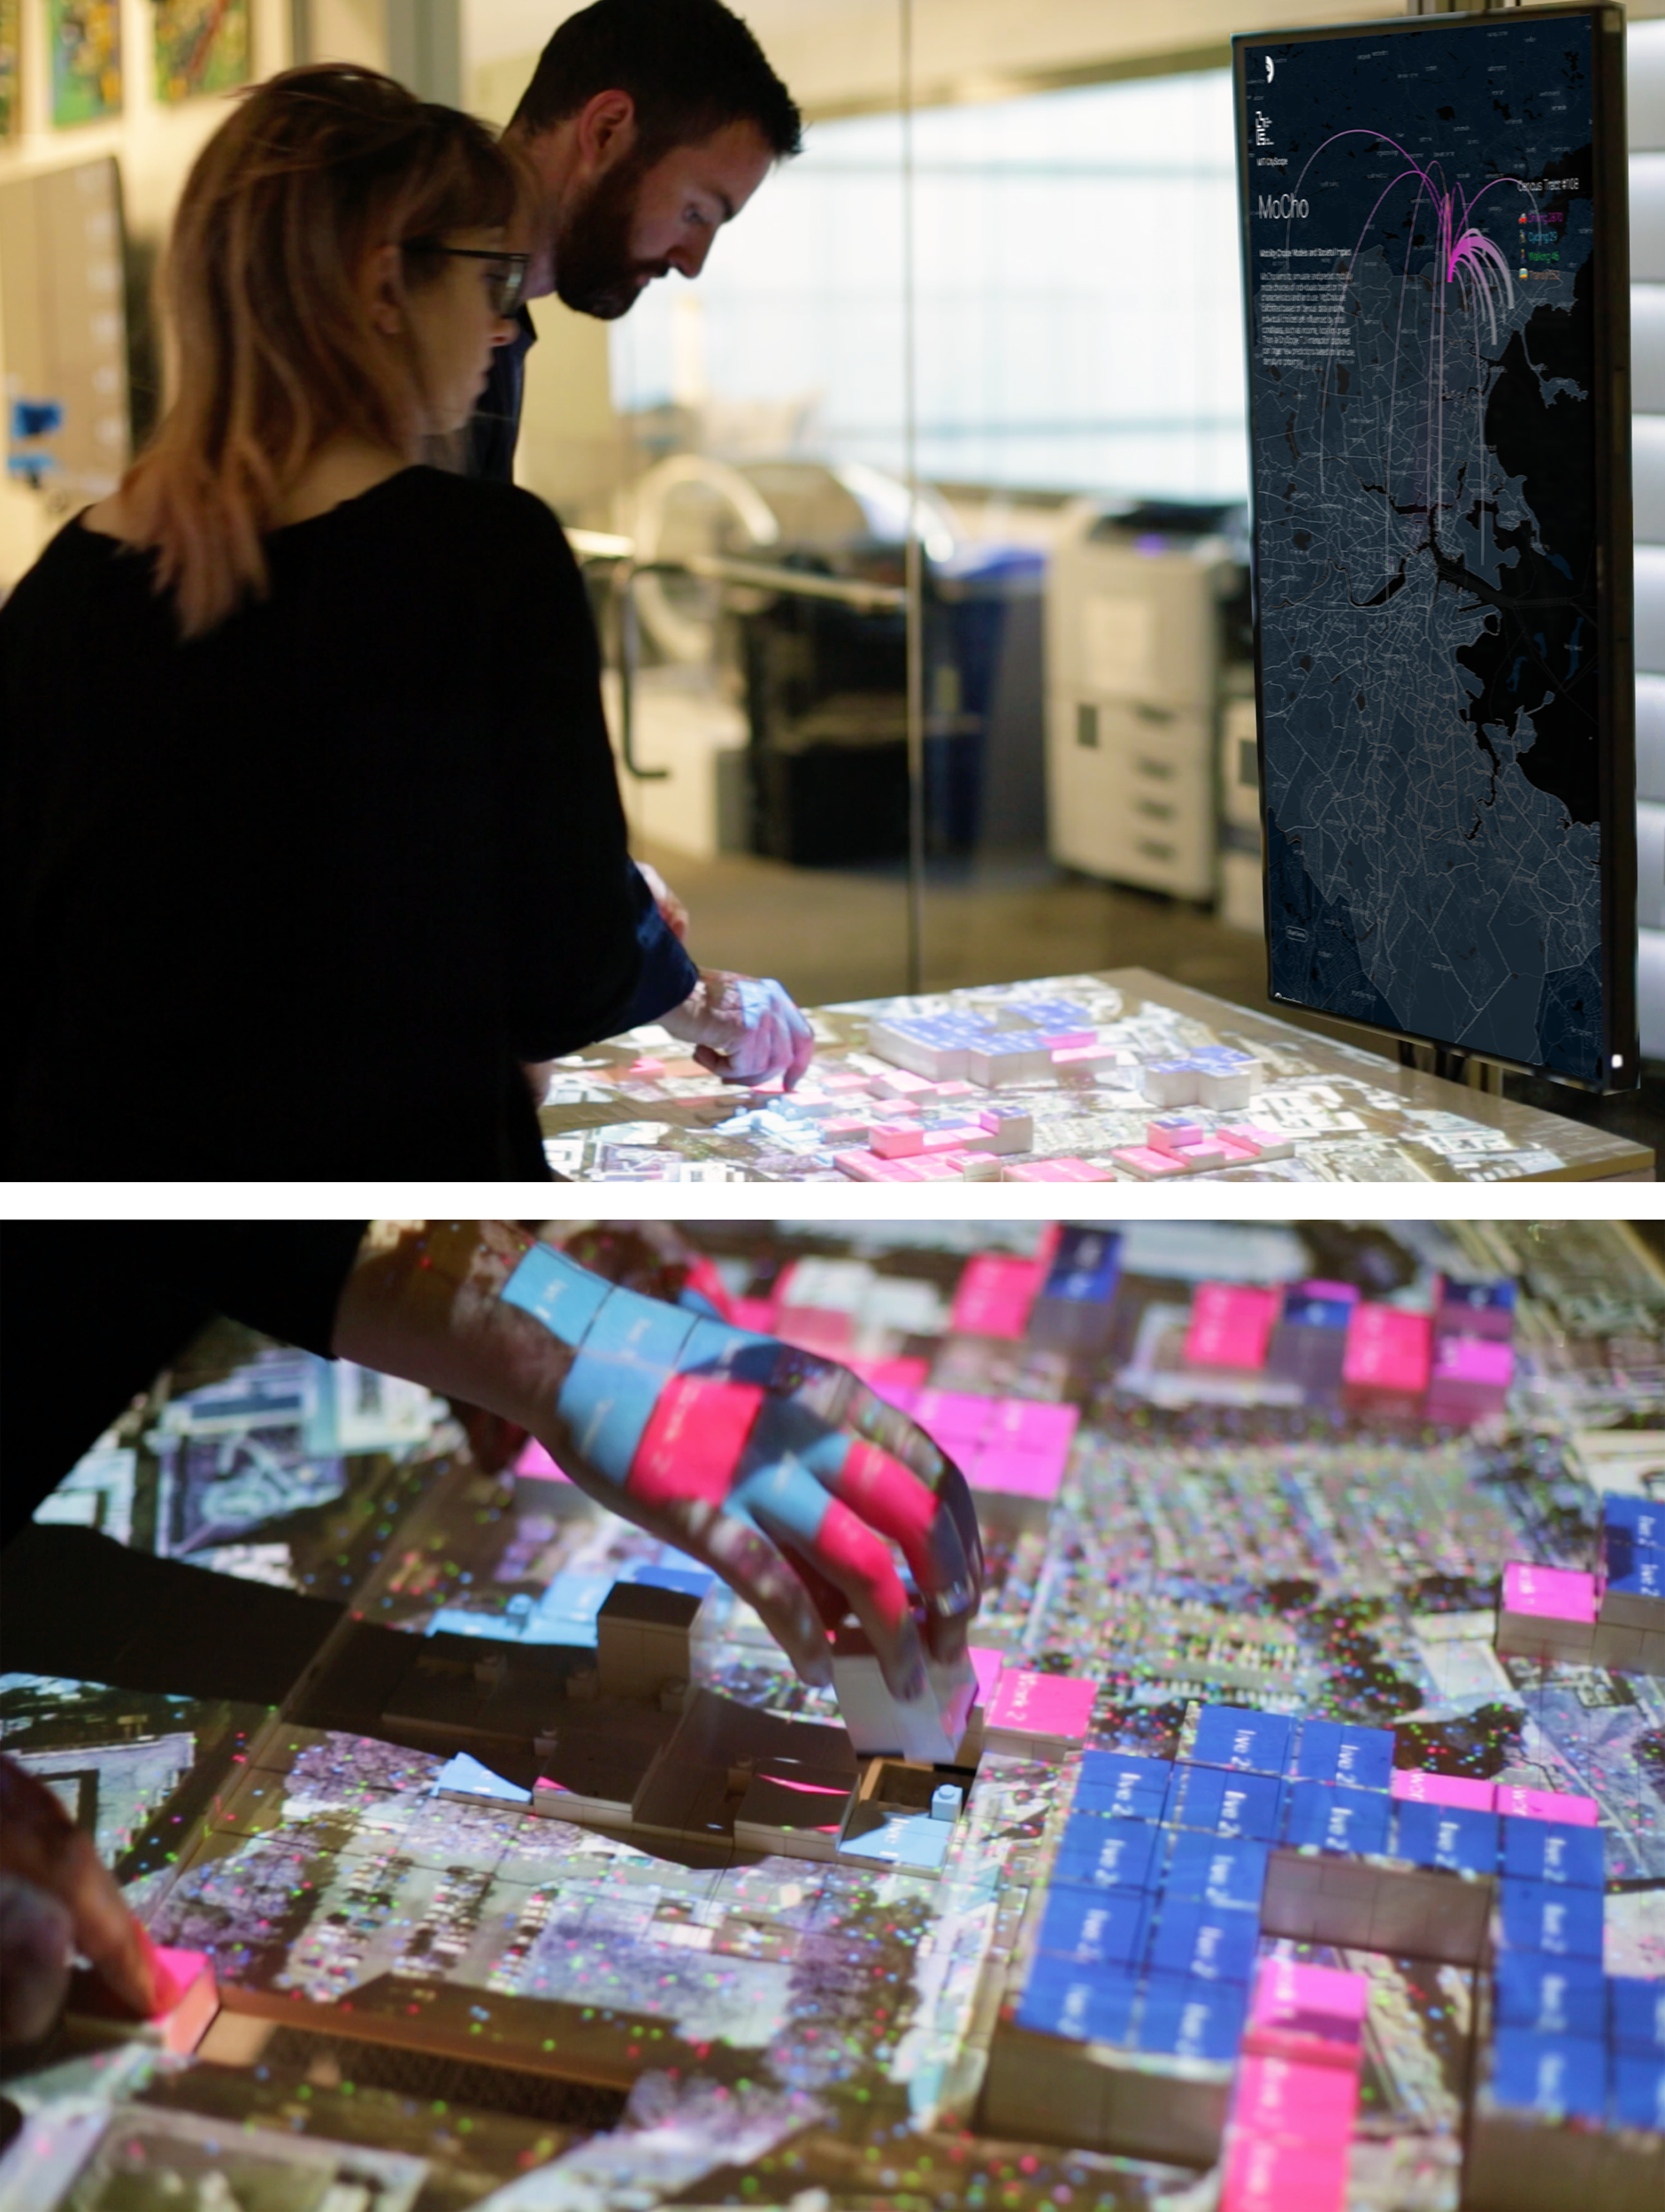
\includegraphics[width=.7\linewidth]{chapters/prediction/mocho/figures/mocho2.png}
        \caption{
            MoCho and CityScope TUI. Interaction results are computed and visualized on both vertical (metro-scale) and horizontal (parcel-scale) planes. A TUI slider (bottom left corner) allows density and building-height iteration for the land-use type used as the slider handle.
        }
        \label{fig:mocho_tui}
    \end{figure}

    \subsection{Motivation}
    {
        The individual choices urban dwellers make about their mobility and transportation behavior have profound impacts on their own lives, as well as on society as a whole. Motorized transportation leads to negative external impacts such as carbon emissions and air pollution, whereas active mode-choices such as walking and cycling improve the physical and mental health of travelers \cite{doorley2015quantifying, mueller2015health}. Urban-planning can influence these mobility choices and their societal impacts by organizing spatial land-uses and infrastructure to encourage short trips using active modes \cite{handy2002built, saelens2003environmental}. Statistical learning methods have been used successfully both in research and in practice to predict the mode-choices of travellers in response to urban interventions \cite{ben1999discrete, wardman2007factors, habib2009investigation, buehler2016bikeway}.
        \newline
        Making predictions through statistical models, generally involves the combination of various computing platforms\footnote{Most commonly in R \cite{hasan2014fast}, Stata \cite{gu2013fitting}, specialized transportation modeling software such as SimMobility \cite{adnan2016simmobility} or Python and GIS plugins.}. These may carry steep learning curves, require specialized skills, and feature limited capabilities for real-time interaction \cite{ben-joseph2001}. In this study, a CityScope instance was devised to overcome these challenges using a combination of real-time statistical models with an interactive, real-time user interface.
    }

    \subsection{Data and Modeling} \label{sec:mocho-models-data}

    {
        MoCho makes use of publicly available datasets which cover major urban areas in the US; This ensures that the methodology presented here can be replicated for the vast majority of American cities. The main data resources used are specified in Table \ref{tab:mocho-dataSources}.

        \begin{table*}[!tb]
            \centering
            \begin{adjustbox}{width=\textwidth}
                \begin{tabular}{ll}
                    \hline
                    \textbf{Resource}                              & \textbf{Description}                                                               \\
                    \hline
                    Public Use Microdata Sample (PUMS)             & Individual person and household level survey data for the USA                      \\
                    American Community Survey (ACS)                & Aggregated demographic data for administrative zones in the USA                    \\
                    OpenStreetMap (OSM)                            & An open-source editable map of the world \cite{haklay2008openstreetmap}            \\
                    Open Source Routing Machine (OSRM)             & An API which provides routing information using OSM data \cite{huber2016calculate} \\
                    Open Trip Planner (OTP)                        & A server which computes multi-modal transport itineraries \cite{OTP}               \\
                    Census Transportation Planning Products (CTPP) & A special tabulation of the ACS data for commuting characteristics                 \\
                    \hline
                \end{tabular}
            \end{adjustbox}
            \caption{Data resources used for US cities in CityScope MoCho}
            \label{tab:mocho-dataSources}
        \end{table*}

        These data sources are used to generate a synthetic population and to calibrate a model which could predict their mobility behaviors in response to changes, such as new residential or commercial development. The modeling can be described in four steps: (i) Population synthesis; (ii) Home and job location choices; (iii) Transportation mode-choice; and (iv) Impact assessment. Each of these steps is outlined below.
    }

    \subsubsection{Population Synthesis}
    {
        Mobility behaviors can be analyzed using two main approaches: (i) An aggregate approach, which divides the area into zones and predicts aggregates inter-zonal flows, or (ii) A disaggregate approach, which recognizes that urban mobility patterns are the result of many decisions made by individuals. The disaggregate approaches directly explain why an individual makes a choice given their circumstances, and therefore they are better able to predict how those choices may change in different circumstances \cite{koppelman2006self}. Due to privacy and data availability constraints, it is generally not practical to make predictions with respect to real population. Instead, it is common practice to use population synthesis techniques in order to produce a \textit{Synthetic Population}, and to make predictions with respect to these individuals. The methods take individual household-level demographic profiles and zonal aggregate demographic data, and allocate the individual records to zones in order to create the synthetic population. Some common techniques include Iterative Proportional Fitting \cite{beckman1996creating, guo2007population}, convex optimization \cite{vovsha2015new}, and Bayesian methods \cite{sun2015bayesian}.
        \newline
        The PUMS survey data used here includes the home Public Use Microdata Area (PUMA) and place-of-work PUMA for each respondent, where each PUMA corresponds to a set of census tracts. In order to model commuting trips at a tract-to-tract level, the population synthesis process needs to allocate each individual to a home and work census tract pair. A simple Bayesian method is utilized for this purpose, using the origin-destination flows from the CTPP data as well as aggregate demographic data from the ACS. PUMS individuals with attributes $A$, home PUMA $H$ and work PUMA $POW$ are assigned to an origin-destination (O-D) pair $w_{ij}$ according to the probability calculated with equation \eqref{mocho-eq-bayes}.

        \begin{equation}\label{mocho-eq-bayes}
            P(w_{ij}|A)\propto\delta_{ij}\prod_{a \in A}P(a|w_{ij})P(w_{ij})
            \\
            \quad where
            \\
            \quad
            \delta_{ij}=
            \begin{cases}
                1, & \text{if}\ H\subset i \text{ and } POW\subset j \\
                0, & \text{otherwise}
            \end{cases}
        \end{equation}

        The prior probabilities $P(a|w\_{ij})$ and $P(w\_{ij})$ may be obtained from the ACS aggregate demographic data and the CTPP O-D data.
    }

    \subsubsection{Home and Employment Location Choices}
    {
        MoCho aims to simulate the changes in home and work locations in response to amended land-use, density and spatial organization. It was assumed that when a residential or employment unit appears in a census tract, new residents or workers also appear. The number of new people is determined by the density of the unit; some demographic attributes, such as income or job sector, may be determined by the unit type. It is also assumed that the conditional probability distribution of the new residents' demographic attributes and work locations, is similar to that of the existing residents of that same tract, conditional on the known attributes. Therefore, the new resident can be simulated by cloning a randomly sampled person with the same home location tract and attributes from the synthetic population. A similar process is used to assign home locations to new workers; This location choice can be expected to be accurate for small changes to the land-uses and densities in a district but for more substantial changes, a more sophisticated model may be required.
    }

    \subsubsection{Mode-Choices}\label{sec:modeChoices}

    {
        The choice of transportation mode for each synthetic individual's commute should be predicted in response to each intervention. The mode-choices (MC) are modelled using a logit-based discrete choice model\footnote{Discrete choice models has been used extensively by researchers and practitioners in modeling of decisions including home location, work location and mode of transportation. An advantage of discrete choice models over other classification models is that their estimated parameters have economic interpretations; This means that the final model results can be easily understood by practitioners \cite{train2009discrete}.}. Discrete choice models assume that individual decision-makers select the alternative which maximizes their utility from their available options.
        \newline
        The utility is composed of a systematic component and a stochastic component: The systematic portion of the utility is (i) an additive function of attributes of the decision maker, (ii) attributes of the alternative, and (iii) interactions between both. This stochastic component is needed because in reality, two people with the same measured attributes may take different decisions when faced with similar alternatives. This component is typically assumed to be Gumbel distributed due to computational advantages and this leads to the logit formulation. These models can be defined by the following expressions \cite{koppelman2006self}:

        \begin{equation}\label{dcm}
            %   \begin{aligned}
            U(X_i, S_t)\geq U(X_j, S_t) \forall j \in C
            \quad \text{and}\quad
            U_{it}=V_{it} + \epsilon_{it}
            \quad \text{and}\quad
            V_{it}=V(S_t)+V(X_i)+V(S_t,X_i)
            %   \end{aligned}
        \end{equation}

        where $C$ is the choice set, $i$ is the alternative chosen by decision maker $t$,  $U_{it}$ is the true utility of alternative $i$ to decision maker $t$, $X_i$ are the attributes of option $i$, $S_t$ are the attributes of person t, $V$ is the systematic utility and $\epsilon$ is the stochastic utility.
        \newline
        The parameters of the logit model must be calibrated with individual-level stated-choice or revealed-choice data. For MoCho, individual observations from the PUMS data could be used for this calibration. The PUMS survey data contains 12 different options for MC but for the purpose of this work, this list is simplified to 4 major modes: car, bicycle, walk and public transportation modes. The explanatory variables considered for inclusion in the model include person attributes from the PUMS data (such as: age, income, gender, education level and employment type), attributes of the home and workplace census tracts from the ACS data, and the estimated travel times and costs for each mode and each trip. The travel times for each census tract pair were estimated by querying the OpenStreetMap API (for walking, cycling and driving times) and Open Trip Planner (for public transit travel times) \cite{OTP}. The PUMS data and ACS data contain hundreds of variables and so some exploratory analysis and feature engineering needs to be done to create a list of candidate features prior to model fitting. Once the features have been selected, the coefficients of each features can be estimated by maximum likelihood estimation, in this case using the python library `pylogit'.
    }


    \begin{figure}[!htb]
        \centering
        \includegraphics[width=.75\linewidth]{chapters/prediction/mocho/figures/mocho0.png}
        \caption{Software architecture. The CityScope table data is sent to cityIO from the tangible interface made with LEGO. cityIO stores that data to have it available to the MoCho computation module. MoCho combines this data with other geo-data from the Geo server and performs computation. The Frontend visualizes the table state and mode-choices. Each arrow indicates an HTTP response.}
        \label{fig:mocho_arch}
    \end{figure}


    \subsection{System Architecture}

    {
        CityScope MoCho is designed to allow decision-makers, planners and community members to experiment with different land-uses and spatial organizations, and understand their impact on mobility choices. As described in Section \eqref{sec:cityscope_architecture}, MoCho included cityIO, CityScope Schema, and and an early version of the CSjs frontend. It practiced the principal concept of separating frontend, backend, and microservices, and it was allowing the parallel development and maintenance of each component independently. Nevertheless, MoCho was still lacking the flexibility of later CityScope architecture, such as in the previously discussed Grasbrook project (see Section \eqref{sec:grasbrook}).
        \newline
        In this case study, the system setup consists of a CityScope TUI, including a tabletop 3D urban model, a projection scheme, and other feedback devices. The software, illustrated in Figure \eqref{fig:mocho_arch}
        consists of four parts: (i) TUI and frontend; (ii) Data management; (iii) Backend computation for the MC model; and (iv) A spatial Geo-Server. The rest of the section describes each of the system's different components, the data-flow and networking between them.




        \subsubsection{User Interaction}
        {
            MoCho uses CityScoPy \eqref{subsec:csarch-cityscopy} to recognize monochromatic tags over a uniform grid. Added to this project were TUI sliders constrained on one axis and scanned along an indentation. Unlike other tiles, slider emits a float value ($0 - 1$) that is added to the rest of the grid data and transmitted to cityIO server \eqref{subsec:csarch-cityio}. A feedback module contains display screens and projectors communicate the analysis outcomes back to the user.
        }
        \subsubsection{cityIO}
        {
            MoCho used an early version of the CityScope microservices architecture. The MoCho API (described in Section \eqref{sec:mocho_api}) listens to cityIO to attain the TUI state, and combines it with data from the Geo-Server to make MC predictions. The flow of data within this system has four steps: (i) The TUI interface reads the tags and sends them via HTTP request to cityIO; (ii) cityIO receives the CityScope data and exposes it to MoCho API; (iii) In combination with the data from the Geo-Server, MoCho predicts and exposes the result by it's own HTTP endpoint; (iv) The CSjs frontend collects data from the different APIs and visualizes the overall result on the CityScope instance.
        }
        \subsubsection{MoCho API}\label{sec:mocho_api}
        {
            The MoCho API is the module responsible for predicting the mobility choices of each simulated individual, in response to changes to the state of the TUI data. When a change is detected, the module creates new synthetic population corresponding to the amended residential or commercial buildings, and assigns their home and work locations as described in Section \eqref{sec:mocho-models-data}. The residential and employment densities of the tracts containing the new buildings are also updated. The modes of transportation for each commuting trip are then predicted using the MC model. The results are sent as JSON format and are exposed to the CSjs frontend for visualization.
            \newline
            User interactions can lead to changes in the mobility choice and impact predictions in three ways: First, when residential and commercial units are added to denser, more central parts of the city, the newly spawned individuals will be more likely to choose workplaces with shorter commutes. Second, when new units are added to parts of the city where the current population of residents/workers has personal characteristics which tend to favor alternative mode (cycling for example), the newly spawned people will tend to inherit those characteristics. Lastly, the addition of new buildings affects the attributes of the census tract, such as overall residential and employment density and these attributes can affect the mode-choice probabilities of all people living and working in the census tract.
        }

        \subsubsection{Geodata API}
        {
            Census tracts and other geo-spatial data are required to compute MC as well as to visualized the prediction. For this purpose, an additional module was designed to service \verb|GEOJSON| data for the study area. In the case study of Section \eqref{subsec:mocho-volpe}, geo-data for the Boston Metro area and for a selected interactive region in Cambridge, MA were served. This API can be easily scaled to serve MoCho or other modules in different regions, given access and availability of spatial data.
        }
    }

    \subsection{Case Study: Volpe}\label{subsec:mocho-volpe}
    {
        To examine the MC model in a real-world mobility environment, a site under development in Kendall Sq., Cambridge MA was selected. A CityScope TUI, a cityIO endpoint, and GeoServer instance were built for this site. This Section will explore the MoCho Volpe instance in details.

        \subsubsection{CityScope MoCho}
        {
            The setup shown in Figure \eqref{fig:mocho_components} was designed for the Volpe site and its immediate surroundings\footnote{Covering a region of $\sim$0.5sqkm at the scale of 1:500, where each 4x4 LEGO-tile represents a 16sqm or 4sqm per each LEGO stud.}. For interaction, six major classes of land-use were defined: open and green spaces, streets, high-income housing ($Housing-1$), mid-to-low income housing ($Housing-2$), large companies' development ($Commercial-1$), and startup and co-working spaces development ($Commercial-2$). Each LEGO tile on the CityScope TUI is classified with one of these land-uses.
            Allocating different tiles next to the each other (e.g., two tiles of type $housing-2$ and one tile of type $commercial-1$) would be translated as a mixed-use structure with multistory housing and offices. The TUI slider adds an additional dynamic control which allows the density (height) of all cells of the same class to be altered concurrently, as shown in Figure \eqref{fig:mocho_components}.
        }

        \begin{figure}[!htb]
            \centering
            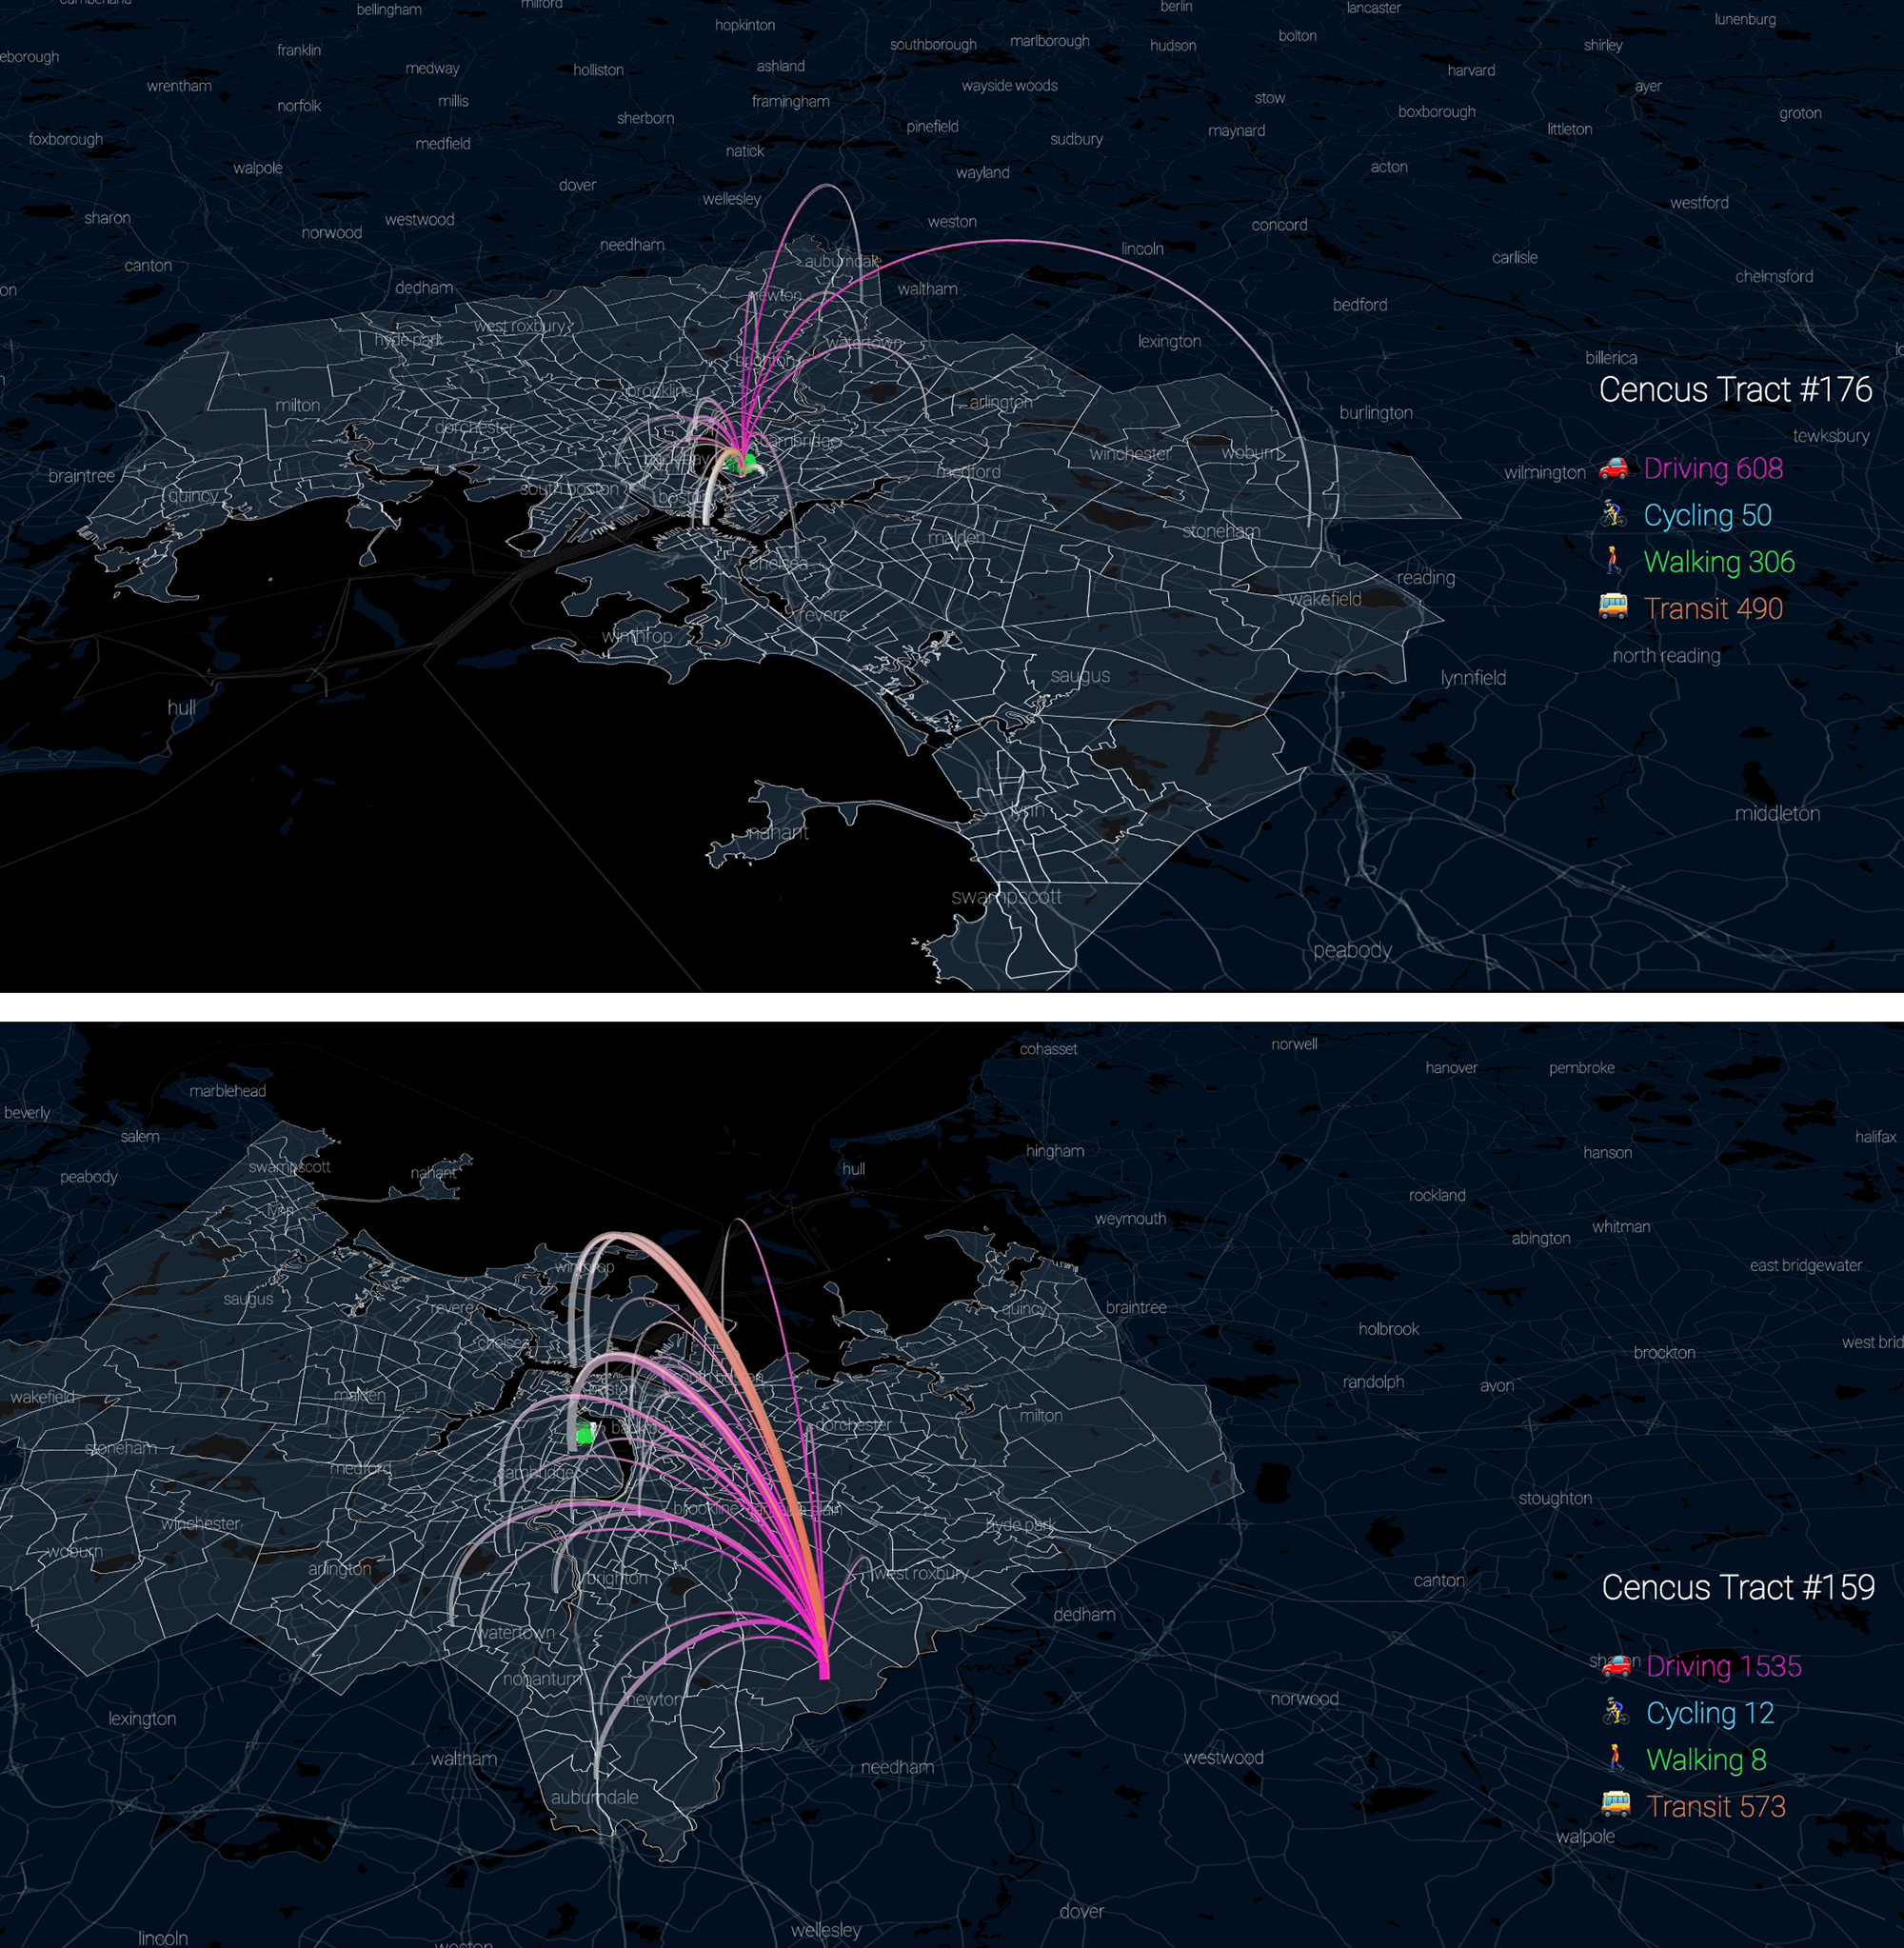
\includegraphics[width=.9\linewidth]{chapters/prediction/mocho/figures/mocho3.png}
            \caption{MC predictions}\label{fig:mocho_arcs}
            \caption*{MC model results. (top) shows trips originating at the Volpe site census tract and (bottom) showing trips from a suburban tracts. The arcs display volumes of trips (thicknesses) between each O-D pair for each mode (color). As clearly shown, the suburban tract yields more car trips with greater distances than those originating at the Volpe site.}
        \end{figure}


        \subsubsection {Feedback}
        {
            This feedback component shows data from the MC model, the scanned TUI and a Geo-data service. The Geo-data service serve census tract data of the Greater Boston Area via \verb|GEOJSON| polygons, projected onto a cartographic background. Than, the results of the MoCho model are rendered as origin-destination (O-D) arcs connecting pairs of different census-tracts, as shown in Figure \eqref{fig:mocho_arcs}. Each arc represents the sum of trips between the pair of tracts, with color representing the prevailing MC chosen by most trips leaving that tract (i.e., green for bikes, purple for cars, etc.). The arc's thickness corresponds to the sum of trips by that mode. On average, nearly 11,000 arcs are reproduced with each user iteration; To avoid illegibility and visual noise, the UI renders only arcs terminating at a given census tract, selected via user's interaction. For each selected census tract, the breakdown of trips by each mode also displayed in numerical format. The UI was built and deployed as a web application, using the ReactJS \cite{react}, Mapbox GLJS, and DeckGL \cite{deckgl17:online}.
        }

        \subsubsection{MoCho TUI}
        {
            The MoCho TUI is used as the design space and a canvas for visualization. With each user interaction, the canvas updates a schematics land-use diagram, representing the Volpe development site. A shadow mapping algorithm adds perceptual depth to the grid tiles so that higher density tiles appear taller than others. A background mapping service contextualizes the design space to the site, in this case Volpe area. Lastly, animated color dots represent individual trips entering or exiting the site, as they are inferred from the MoCho model. The dots colors correspond to the mode-choice arcs on the vertical display (i.e., a purple dot is one vehicular trip) and animated to move from general direction of that tract to its designated land-use destination.
            \newline
            A more advanced version of this simulation assigns trips to routes based on Dynamic User Equilibrium or micro-simulation, and feed updated travel times back to the mode-choice predictions. This simulation was introduced to the CityScope Grasbrook \eqref{sec:grasbrook} and later in the CityScope Corktown project in Detroit, MI. Together, the feedback modules assist users to associate the relatively small-scale urban development with metro-scale MC impacts.

            \begin{figure}[!htb]
                \centering
                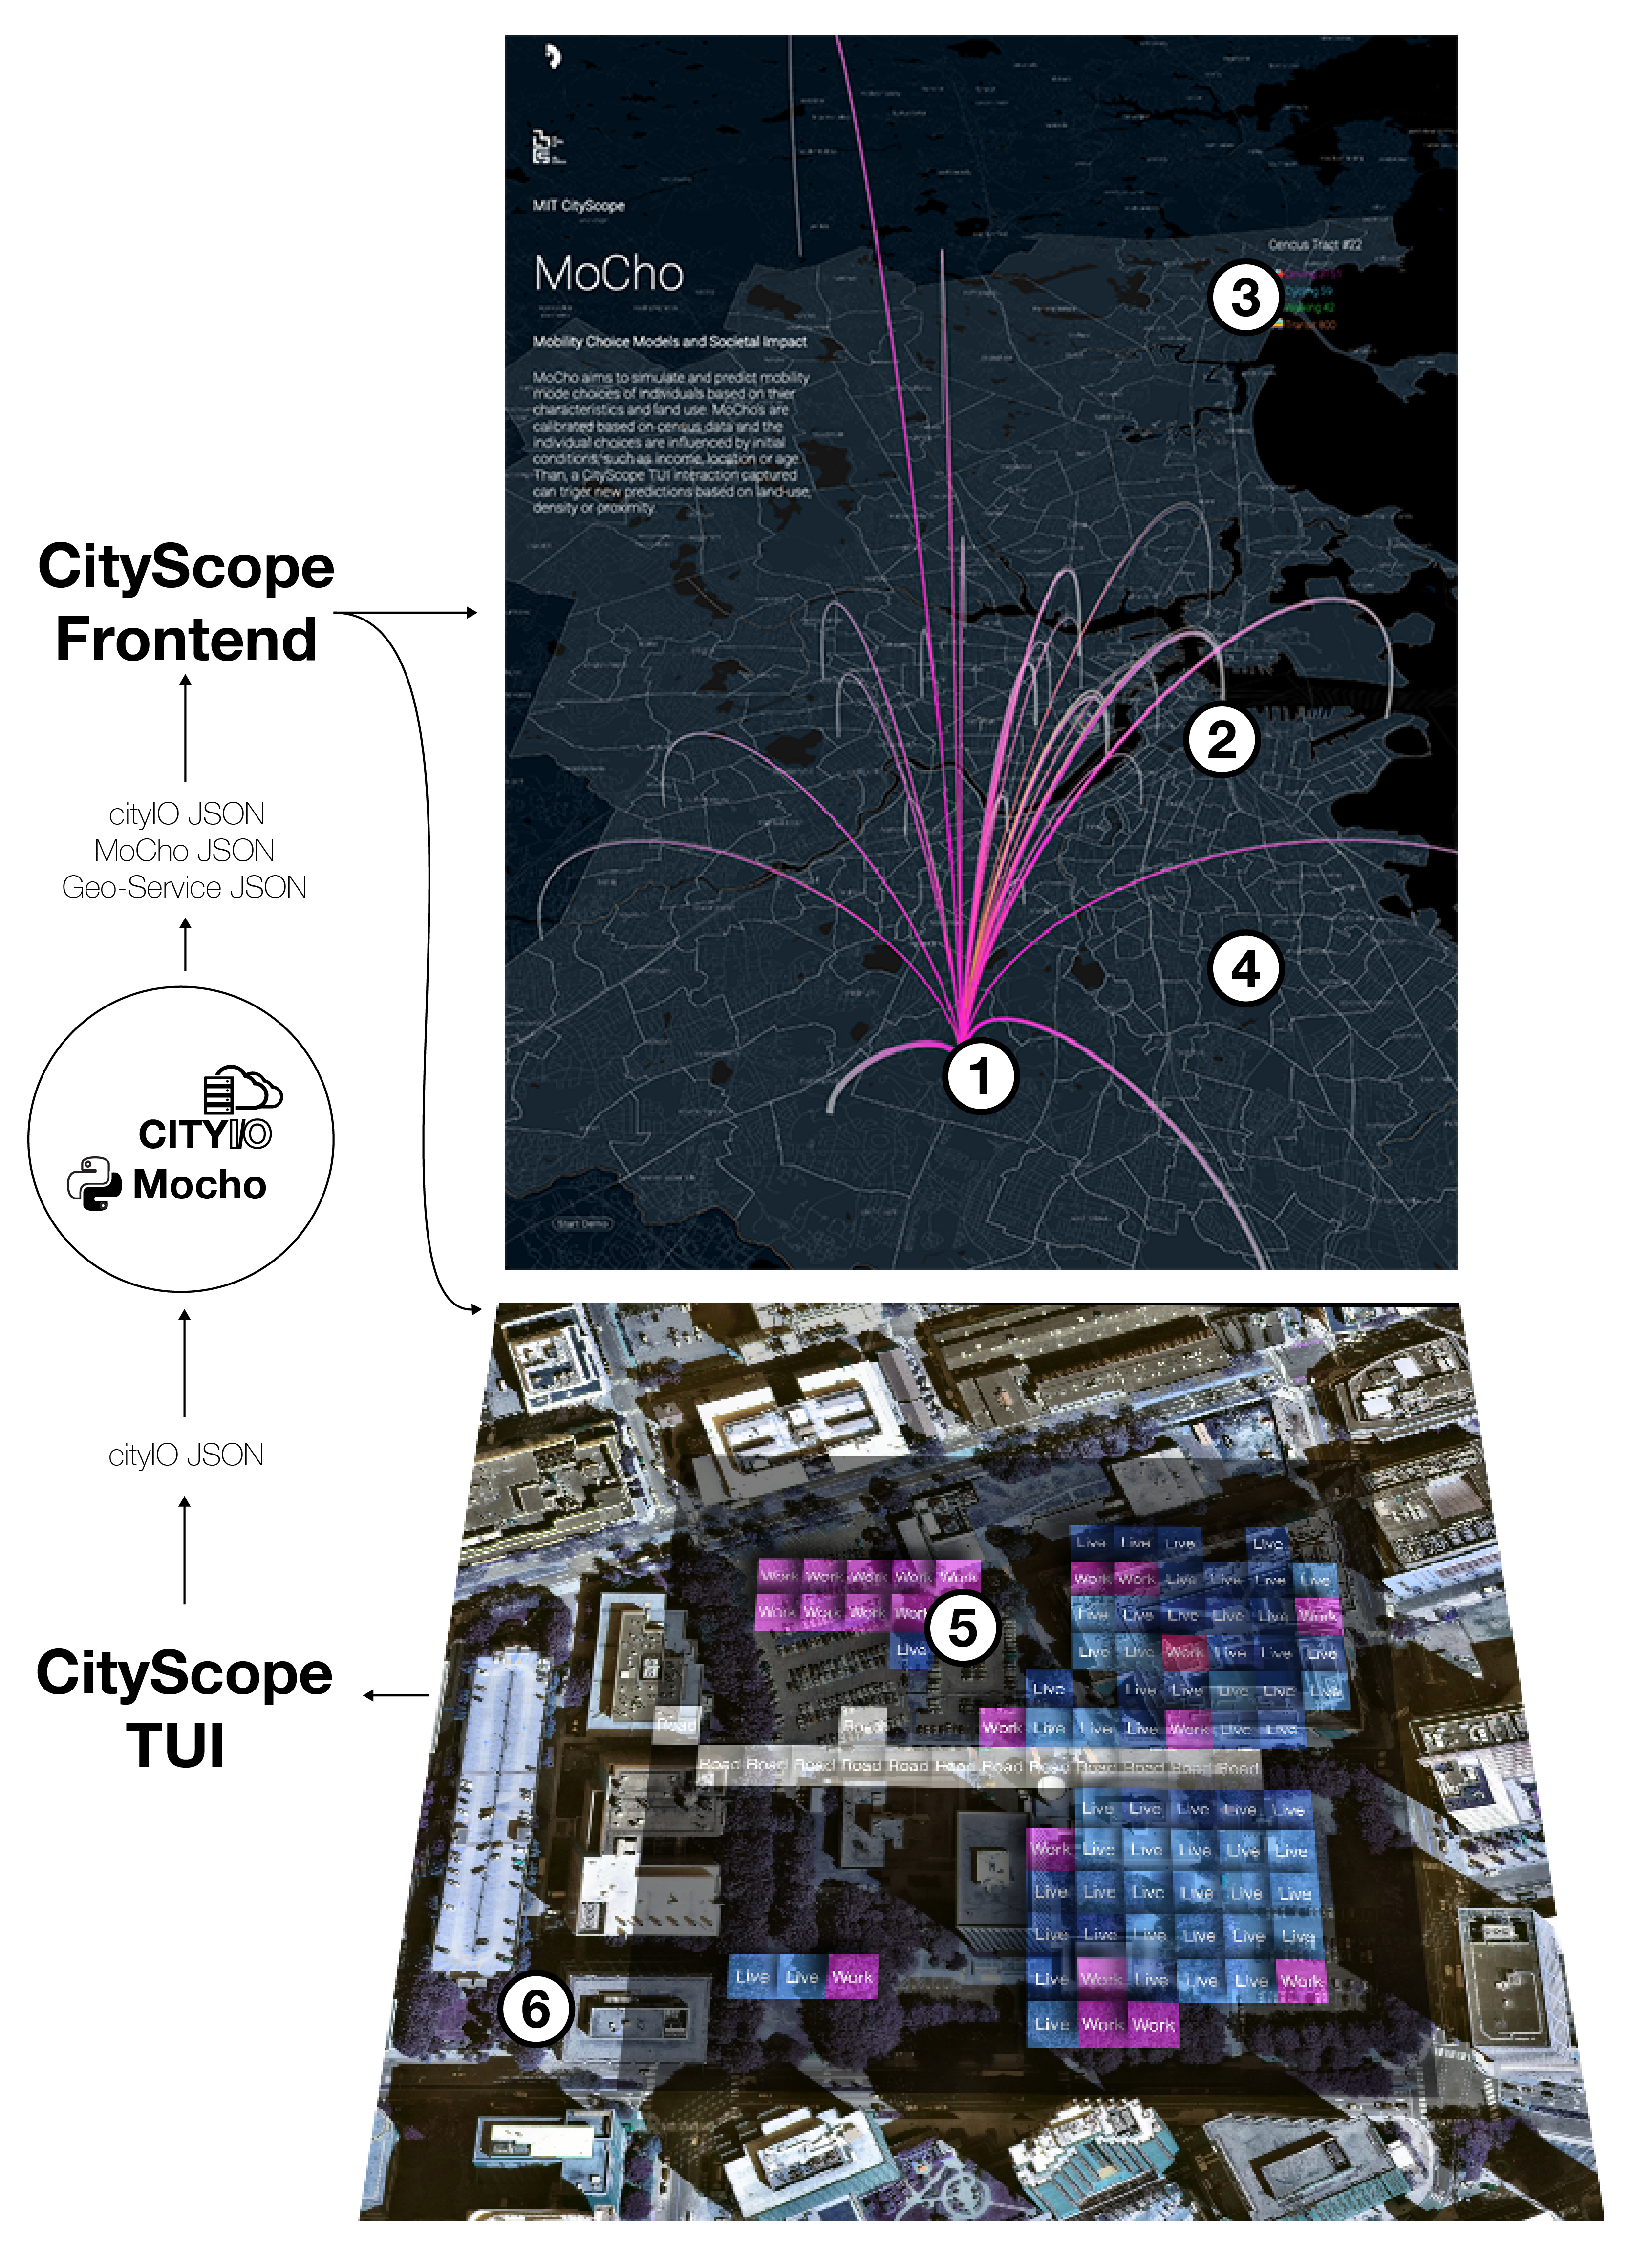
\includegraphics[width=0.65\linewidth]{chapters/prediction/mocho/figures/mocho1.jpg}
                \caption{CityScope MoCho Interface Components}\label{fig:mocho_components}
                \caption*{Vertical Display: (1) Selected tract showing trips and their MC (2) MC trip ending at the Volpe site (3) Numerical output of tract's MC (4) GeoJson of ~500 computed census tracts. Horizontal TUI: (5) Tagged LEGO bricks with projected land-use scheme (6) Immediate context surrounding the Volpe site design space}
            \end{figure}

        }

        \subsubsection{Model Calibration Results}
        {
            The mode-choice model introduced in Section \eqref{sec:mocho-models-data} must be calibrated for each location context; For the Volpe Case Study, data for the Boston metro area were used. Through some exploratory analysis of Boston's PUMS data, a number of variables were selected as being likely to affect MC. As well, some features were converted to different formats. For example, the age and income variables were converted from continuous to binary variables by dividing each into three quantiles and using binary variables to indicate records in the lowest and highest groups.
            \newline
            The encoding of travel-time also required some experimentation. Time spent in different types of travel activities, such as driving, waiting for a bus or walking, are associated with different perceived costs and therefore should be treated differently in discrete choice models, without being too specific which can cause model under-fitting. In this case study, it was found that using the three variables of \verb|walking\_time|, \verb|cycling\_time| and \verb|in\_vehicle| led to a well fitted model with sensible parameter estimates.
            \newline
            The final model had a pseudo-R-squared value of 0.45 which indicates a well fitting model. The full list of parameters estimates is shown in Appendix Table \eqref{appendix:mocho-tab-results}. When interpreting the parameters, it should be noted that the choice of driving was taken as the reference choice. For example, all of the parameters for the density variables are positive, indicating that increases in residential or employment density in one's home or workplace, are associated with increased likelihood of cycling, walking or public transit relative to driving. The travel-time parameters show that time spent cycling is perceived as the most costly whereas time spent in vehicles is the least costly, which is in line with prior research \cite{koppelman2006self}. Finally, some societal and cultural associations are found between personal characteristics and the likelihood of taking each mode. For example, the model shows that having a college degree, a graduate degree and/or working for a non-profit, decreases one's likelihood of driving and in particular, increases one's likelihood of taking active modes. Also, those in the youngest age group and lowest income group are less likely to drive than others.
        }
    }
    \subsection{Discussion}
    {
        CityScope MoCho was designed to bridge the gap between smilingly minor changes to the built environment, and behavioral choices of individuals in remote locations. It was achieved by predicting mobility choices (MC) and societal impacts in response to user inputs through the CityScope TUI. While there already exist tools for predicting MC and environmental impacts of transportation, few efforts have been made to integrate these modeling steps in an end-to-end real-time, and collaborative tool.
        The underlying models were well calibrated using publicly available data sources, ensuring the credibility of the model predictions; Similar models could be created for other urban areas with minor adaptations to the underlying model.
        \newline
        Moreover, using these models for prediction, typically requires laborious specification of inputs by professionals. The platform developed here provides an intuitive user-interface to such models, allowing multiple people with varying levels of expertise to collaboratively experiment with different urban-designs scenarios and real-time feedback. MoCho has advanced the CityScope architecture with on-demand pre-trained models, a distributed computational backend, and an online user interface which was a precursor to CityScopeJS (see Section \eqref{sec:cityscope_architecture}); many of these ideas evolved into the current CityScope platform.
    }
}